\begin{figure}[!htb]
    \centering
    \Subfigure[0.5]{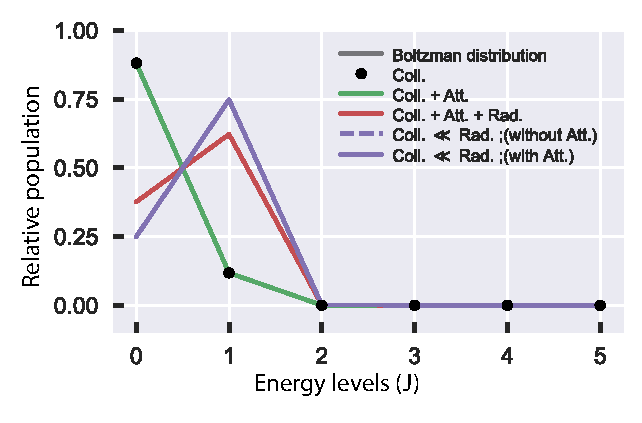
\includegraphics[width=1\textwidth]{figures/simulations/ROSAA/boltzman/CD+_He_f-time__transition_0-1_0.001s_boltzman_comparision.pdf}}{At $t=0.001s$}{\label{fig:thz-sim:boltzman-comparision:1ms}}
    \hfill
    
    \Subfigure[0.48]{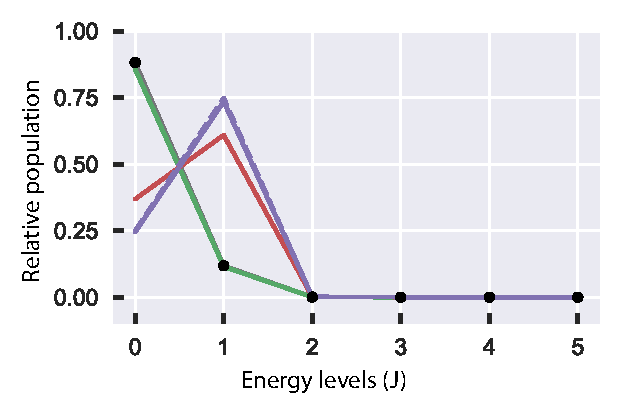
\includegraphics[width=1\textwidth]{figures/simulations/ROSAA/boltzman/CD+_He_f-time__transition_0-1_0.6s_boltzman_comparision.pdf}}{At $t=0.6s$}{\label{fig:thz-sim:boltzman-comparision:0.6s}}
    \hfill
    \Subfigure[0.48]{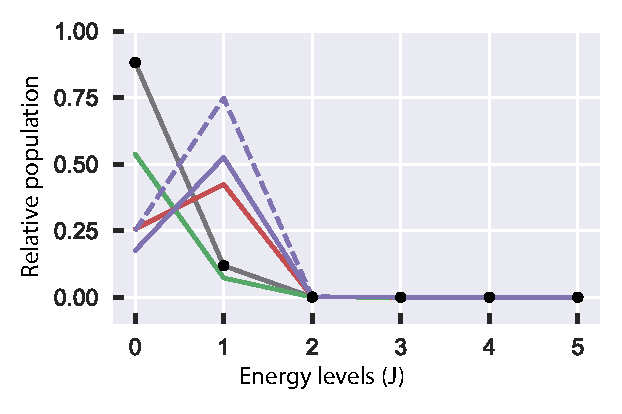
\includegraphics[width=1\textwidth]{figures/simulations/ROSAA/boltzman/CD+_He_f-time__transition_0-1_100.0s_boltzman_comparision.pdf}}{At $t=100s$}{\label{fig:thz-sim:boltzman-comparision:100s}}
    % \hfill
    \caption{Relative population of rotational energy levels ($J$) from the numerical simulation at the time ($t$) indicated under the caption. The simulation conditions are as follows: T$_{coll}=7$ K, $a=0.5$, Helium number density $2.2 \cdot 10^{14}$ \percc\ and radiation power $3.5\cdot10^{-5}$ W. Different process are colour coded and labelled in (a), are compared with Boltzmann distribution (black solid line) at T$_{coll}=7$ K.  The labels indicate the following process as only collisional (Coll.), collisional process with He attachment (Coll. + Att.) and Rad. indicates the presence of a radiative process, Coll. $\ll$ Rad. indicates that the radiative process rates are much larger ($>10^{5}$ higher) than collisional rates.}
    \label{fig:thz-sim:boltzman-comparision}
\end{figure}